\chapter{Métodos contra Trapaças em Jogos Online}
\label{cap:metodologias}

Diferentes métodos podem ser empregados para evitar ou detectar trapaças que usuários mal intencionados estejam utilizando. Focando em um conjunto mais restrito de trapaças, mais especificamente, as apresentados no Capítulo \ref{adulteracao}, diferentes estratégias podem ser abordadas para se prevenir. Dois destes métodos, abordados em estudos anteriores por \cite{NVE} e \cite{implementacaosimbolica}, são explicados nos Capítulos \ref{simbolics} e \ref{semantics}, e implementados nos Capítulos \ref{implementsimbolic} e \ref{implementsemantic}.

\section{Verificação do Executável}
É notório que uma das formas de executar trapaças é alterar o executável do jogo, modificando dados de atributos do personagem, ou permitindo que determinadas ações inicialmente proibidas sejam possíveis de serem executadas. 
Uma das formas de evitar isso é checar periodicamente a conformidade do executável do usuário. Por exemplo, o cliente do jogo, antes de possibilitar que o usuário se conecte ao jogo com sua conta, utiliza um verificador no executável do usuário e o compara com um executável válido. Uma estratégia é a utilização de uma \textit{hash} criptográfica, que permite a compressão unidirecional (compressão que não pode ser revertida) do executável do cliente, que é então enviado ao servidor e comparada com a \textit{hash} previamente criada de um executável confiável. Se forem compatíveis, conclui-se que o usuário não alterou seu cliente de jogo. Esta estratégia, entretanto, ainda não resolve outros problemas encontrados em um cliente sem autoridade. Outros programas de terceiros ainda podem interagir com as informações que se encontram na aplicação, possibilitando que ações inválidas ocorram se o servidor não averiguá-las. 


\section{Cliente sem autoridade sobre o estado do servidor}
A estratégia adotada mais comum para se prevenir de maus comportamentos dos clientes é garantir que o cliente não possua estado de autoridade que possa afetar o servidor ou a aplicação. O básico dessa abordagem é enviar ao servidor todos \textit{inputs} do cliente, que são executados e validados diretamente no servidor. Esta estratégia não se preocupa com o processamento extensivo realizado no servidor, afinal, nenhum processamento crítico é executado no computador do cliente. Pode-se categorizar este tipo de estratégia como inviável para aplicações com custos computacionais significativos ou com público alvo grande, o que é o caso para a maioria dos jogos \textit{online} encontrados atualmente. Para jogos onde o tempo de resposta não é impactante na experiência proporcionada aos jogadores, como em jogos de turnos de estratégia, esta opção pode ser considerada viável. Jogos de xadrez \textit{online} ou jogos de cartas, por exemplo, são estilos de jogos que não são afetados tão negativamente pelo tempo de resposta maior do servidor. 

\section{Validação por outro cliente}

O servidor pode agir como o meio de comunicação entre dois clientes, fazendo com que outro jogador valide a mensagem enviada. Nesta estratégia, a validação ocorre diretamente na aplicação de outro usuário que retorna ao servidor se a ação é considerada válida ou não. Apesar do custo computacional acontecer diretamente no cliente, e na maioria dos casos, esse processamento ser insignificante isoladamente e rápido, o número de mensagens de uma ação é dobrada. Para cada mensagem enviada do cliente ao servidor, outras duas novas mensagens devem ser transmitidas, do servidor ao cliente dois, e novamente do cliente dois ao cliente um. Outro problema é a divulgação de informações que o jogador poderia não ter acesso. Em uma situação onde o cliente 2 recebe informações do cliente 1 para validar, ele acaba ganhando acesso aos dados a serem verificados. Em cenários onde existem informações confidenciais a outros jogadores, esta estratégia não é muito útil, pela necessidade da quebra de confidenciabilidade sobre os dados a serem verificados.


\section{Validação com Execução Simbólica}

\label{simbolics}

A execução simbólica é uma das formas de analisar um programa e determinar quais entradas dele causaram a execução de cada parte do programa. Em vez de utilizar valores de entrada concretos, como números inteiros ou de ponte flutuante, os valores são transformados em valores simbólicos, e, como eles, sua saída é gerada simbolicamente. Seu uso mais convencional é no teste de \textit{software}, utilizado na análise de erros. Nessa análise, as entradas e condições que acarretaram a ocorrência dos erros são previstas utilizando a execução simbólica. 

A execução simbólica utiliza o paradigma Programação com Restrições, que consiste em especificar quais critérios (definidos formalmente como restrições) uma solução deve cumprir. Um resolvedor de restrições então utilizará as restrições especificadas juntamente com o fluxo lógico do programa para descobrir quais valores concretos de entrada gatilharam a ocorrência dos erros.

A Ilustração \ref{fig:exsimb} representa o fluxograma gerado após a execução simbólica de \textit{x}. No exemplo, verifica-se se \textit{x} é maior que zero, e depois, se \textit{x} é maior que dez. No primeiro teste, dois fluxos de execução podem acontecer: ou \textit{x} é maior que zero, ou não. Em cada um destes novos fluxos de execução, é verificado se \textit{x} é maior que dez. No segundo fluxo, a hipótese de \textit{x} ser maior que dez é descartada, afinal, \textit{x} mostrou-se menor que zero no teste anterior.  

\begin{ilustracao}
	\begin{center}
		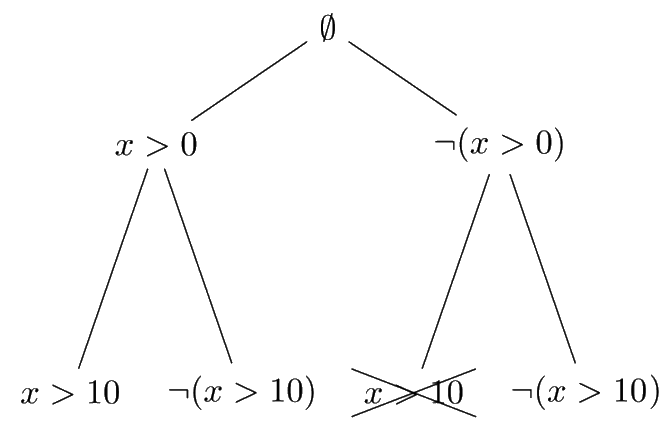
\includegraphics[width=0.6\textwidth]{imagens/exemplosimbolic.png}
		
		\caption[Exemplo de execução simbólica de um programa simples.]{Exemplo de execução simbólica de um programa simples.}
		\fonte{Retirado da apresentação de \citeonline{tixinha}.}
		\label{fig:exsimb}	
	\end{center}

\end{ilustracao}


 \cite{implementacaosimbolica} demonstra um exemplo prático de uma implementação simbólica em um jogo simples.


\begin{figure}[h!]
		\small
		\begin{multicols}{2}

		100: \textit{loc} $\leftarrow$ 0; \\
		101: \\
		102: enquanto true faça \\
		103:\tab    key $\leftarrow$ lekey(); \\
		104:\tab	se key = ESC entao \\
		105:\tab\tab		fimjogo(); \\
		106:\tab	senao se key = '$\uparrow$' entao \\
		107:\tab\tab		loc $\leftarrow$  loc + 1; \\
		108:\tab	senao se key = '$\downarrow$' entao \\
		109:\tab\tab		loc $\leftarrow$  loc -- 1; \\
		110:\tab	fim se \\
		111:\tab envialocalizacao(loc); \\
		112: fim enquanto \\

		\footnotesize
		\textit{(a) Exemplo simples de um cliente}

		\small
		200: \textit{loc\_ant} $\leftarrow$ 0; \\
		201: \textit{loc} $\leftarrow$ \textit{loc\_ant}; \\
		202: enquanto true faça \\
		203:\tab	key $\leftarrow$ simbolico; \\
		204:\tab	se key = ESC entao \\
		205:\tab\tab		fimjogo(); \\
		206:\tab	senao se key = '$\uparrow$' entao \\
		207:\tab\tab		loc $\leftarrow$  loc + 1; \\
		208:\tab	senao se key = '$\downarrow$' entao \\
		209:\tab\tab		loc $\leftarrow$  loc -- 1; \\
		210:\tab	fim se \\
		211:\tab	\textit{breakpoint}; \\
		212: fim enquanto \\ 

		\footnotesize
		\textit{(b) Exemplo instrumentado para executar simbolicamente}

		\end{multicols}

	\caption[Exemplo de execução simbólica com código.]{Exemplo de execução simbólica com código.}
	\fonte{Adaptado de \citeonline{implementacaosimbolica}.}
	\label{fig:codigo1}	

\end{figure}


Neste exemplo simples do jogo Pong \cite{pong} da Ilustração \ref{fig:codigo1}, a aplicação do cliente lê a todo instante as teclas pressionadas pelo usuário, atualizando a posição do jogador de acordo com a direção em que a tecla está pressionada. Em cada iteração do laço principal do programa, o servidor também é atualizado, recebendo a posição atual em que o cliente se encontra. 

Já na versão simbólica do programa, a nova variável \textit{loc\_ant} é instanciada como uma variável simbólica, assim como a variável existente \textit{key}. Um \textit{breakpoint} é criado substituindo a função \textit{envialocalização}, possibilitando que sempre que o fluxo do programa alcançá-lo, se obtenha as restrições geradas em todas variáveis simbólicas. Percebe-se que o envio da mensagem ao servidor não ocorre na versão simbólica, afinal, ela não visa ser uma versão executável tradicional da aplicação, mas sim uma versão que simula os fluxos de operações realizadas durante uma execução.


Para cada escolha gerada na execução do programa, um novo ramo de execução é criado juntamente com uma nova restrição. Essas escolhas são criadas no laço principal, em cada uma de suas iterações. Consequentemente, é possível construir um conjunto de restrições, que representa quais possíveis restrições podem ser geradas em cada iteração do laço principal. 
A partir do exemplo da Figura \ref{fig:codigo1}, dada a iteração \textit{j}, define-se que o conjunto de possíveis restrições que podem ocorrer nessa iteração $C_j$ é o conjunto

\textit{(loc = loc\_ant + 1) $\vee$  (loc = loc\_ant -- 1) $\vee$ (loc = loc\_ant) } \\

Como pode ser deduzido, cada elemento do conjunto $C_j$ depende dos valores anteriores atribuídos a variável \textit{loc\_ant}. Considerando um cenário onde o servidor sabe a última posição do cliente, por exemplo, três possíveis restrições podem ser verificadas na próxima mensagem que o cliente enviar. Caso nenhuma dessas restrições for atendida, ou seja, a variável recebida não for igual, um a mais ou um a menos que o valor anterior, é dedutível que a mensagem enviada pelo cliente é falsa e ele está trapaceando.


\section{Protocolo de Integridade de Semântica Segura}
\label{semantics}

Esta abordagem utiliza um procedimento de auditoria, que é executado por um Servidor de Auditoria. Sua estratégia utiliza o conceito de estados abstratos e concretos na troca de mensagens entre as ações de um cliente. A partir dos estados dos clientes, é utilizado um algoritmo para verificar a integridade da sequência destes estados com a utilização de processos de auditoria.

\subsection {Definição de Estados}
\label{cap:definicaoestado}

Este método utiliza o conceito de estados abstratos e concretos, que são ilustrados na Figura \ref{fig:abstracao}. No exemplo que a Figura \ref{fig:abstracao} traz, duas aproximações foram pensadas para checar se em um determinado vetor \textit{a}, a posição \textit{i} do vetor, \textit{a[i]}, excede os limites do vetor. No primeiro modelo criado, existe um conjunto com todos possíveis valores que \textit{i} pode conter, enquanto que, no segundo modelo, existem possíveis intervalos de valores possíveis que podem conter \textit{i}. Nesta representação simples, é preferível utilizar o segundo modelo, pela sua maior abstração dos valores que \textit{i} pode obter. A primeira aproximação utiliza valores concretos para a resolução do problema, enquanto a segunda utiliza valores abstratos. As setas verdes da figura representam as funções de transformação de domínio que ocorrem de um modelo para o outro.  A transformação $\delta$ representa uma função de abstração (transposição do domínio mais concreto para o mais abstrato), e $\gamma$ representa o processo inverso, uma função de concretização (transposição do domínio mais abstrato para o concreto).

\begin{ilustracao}[h!]
	\begin{center}
		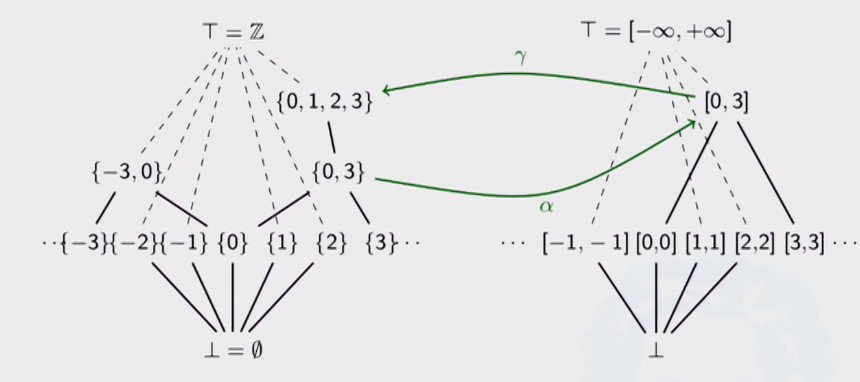
\includegraphics[width=0.6\textwidth]{imagens/abstracao.png}
		\caption[Exemplo da função de Abstração e Concretização]{Exemplo da função de Abstração e Concretização.}
		\fonte{Retirado da apresentação de \citeonline{galoi}.}
		\label{fig:abstracao}
	\end{center}
\end{ilustracao}

Formalmente, define-se que a partir de um estado abstrato \textit{s}, $\gamma$ (s) representa o conjunto de possíveis concretizações que podem ocorrer a \textit{s}. Já um estado concreto S, sua função $\delta$(S) corresponde a um único estado abstrato. Em outras palavras, um estado abstrato pode representar diferentes estados concretos, enquanto que um estado concreto representa um único estado abstrato. Alterações de um estado ocorrem constantemente, e são representadas por $\Delta$, ou \textit{diff}, sendo ele a mudança sofrida de um estado para outro. Em outras palavras, o estado S atualizado para o estado S' sofre a diferença $\Delta$, portanto, S' $=$ S + $\Delta$. 

As funções de transformação de domínio $\gamma$ e $\delta$ podem ser aplicadas não somente nos estados, mas também nas diferenças entre estados. $\gamma$($\delta$), por exemplo, expressa a abstração de uma \textit{diff} $\delta$ qualquer, enquanto $\delta$ representa a concretização da \textit{diff} $\delta$. Algumas conclusões podem ser estabelecidas sobre as \textit{diff}, como $\gamma$(S') $=$ $\gamma$(S) + $\gamma$($\delta$) se S'$=$ S + $\Delta$. Sendo $\alpha$ a representação de uma abstração de uma \textit{diff} $\Delta$ aplicada ao estado S, pode-se deduzir que $\Delta$ $\in$ $\gamma$(S, $\alpha$($\Delta$)) e para cada $\Delta$´ $\in$ $\gamma$(S, $\alpha$($\Delta$)) obtém-se $\alpha$(S $+$ $\Delta$´) $=$ $\alpha$(S´).


\subsection{Aplicação dos estados}

No Protocolo de Integridade de Semântica Segura (SSIP), representam-se as informações do servidor e do cliente em estados, que podem ser tanto abstratos quanto concretos. A representatividade destes estados pode ser encontrada na implementação realizada, referenciada no Capítulo \ref{cap:desenvolvimento}. 

Neste protocolo, o servidor principal da aplicação é denominado Servidor de Estados, que equivale a um servidor convencional de uma NVE, implementado para interagir com os usuários e estabelecer comunicações e trocas de dados sobre as informações do jogo. O servidor de estados contém um estado central abstrato ASTATE, que contém informações relevantes de todos clientes. Imaginando o estado ASTATE como um vetor, por exemplo, cada uma de suas partes é relevante para um cliente conectado a ele. Em outras palavras, de todo estado ASTATE, apenas a parcela ASTATE[$cli_i$] é relevante para o cliente $cli_i$.

Como os clientes possuem estados concretos das informações do jogo, e o servidor possui apenas uma versão abstrata disso,
as funções de transposição de domínios apresentadas no capítulo \ref{cap:definicaoestado} acabam ocorrendo constantemente na comunicação cliente-servidor. Exceto na primeira mensagem de inicialização do cliente com o servidor, por exemplo, todas mensagens posteriores enviadas pelo cliente passam pela função de transposição de abstração. Estas abstrações das mensagens do cliente existem para amenizar o excesso de processamento gerado no servidor nos testes que executa para verificar a validade da mensagem. 

Um exemplo simplificado deste caso encontra-se no jogo implementado \textit{Shooterman} (capítulo \ref{shoterman}). Enquanto variáveis como posição são mantidas no servidor, variáveis de controle mais refinado das ações do personagem são mantidas unicamente no cliente de jogo, como por exemplo, o tempo de recarga de suas ações. Essas informações do estado do jogador são mais abstraídas para o servidor, enquanto são concretas para o cliente do jogador.

Em cada um dos ciclos do cliente, ele envia ao servidor uma abstração $\gamma$ $=$ $\alpha$($\Delta$), que contém uma abstração da \textit{diff} dos últimos estados. Esta abstração é denominada \textit{diff de requisição}. Após o recebimento da \textit{diff} de requisição, o servidor valida a mensagem de acordo com suas semânticas pré-estabelecidas e retorna ao cliente uma confirmação das mudanças requisitadas e das atualizações realizadas pelos outros clientes conectados a NVE. 

Utilizando esta técnica, um cliente malicioso ainda pode violar as regras semânticas estabelecidas pelo servidor, pela susceptibilidade do protocolo, afinal ele só pode verificar se as atualizações abstratas são consistentes com o estado abstrato, sem levar em consideração os valores concretos avaliados. Para solucionar esta falha, ciclos de auditoria são utilizados constantemente para verificar as atualizações de acordo com os estados concretos dos clientes conectados.

\subsection{SSIP}
Outro servidor, denominado Servidor de Auditoria, é utilizado para verificar a integridade semântica dos estados que são constantemente atualizados pelos clientes. Este servidor requisita a um cliente sua sequência de atualizações de estados concretos de um tempo específico junto com seu estado concreto inicial completo, e a partir deles, computa os estados em ordem, verificando sua integridade.

Uma série de operações devem ser seguidas na comunicação do cliente com o servidor de auditoria, e \cite{NVE} dividiu estas operações em três diferentes protocolos, que são apresentados a seguir. Nas ilustrações dos protocolos, são utilizados as setas $\rightarrow$ que representam pacotes enviados de forma não-confiável, e as setas $\hookrightarrow$, que representam pacotes enviados de forma confiável.

\subsection{Protocolo de Inicialização}
\label{protocoloinicializacao}

Este protocolo ocorre quando o cliente inicia seu contato com o servidor. A Figura 3.2 mostra a sequência de passos que deve ser tomada no início da comunicação do cliente com o servidor do jogo.

\begin{figure}[h!]
	\begin{center}
		\fbox{\begin{minipage}{30em}
		\begin{enumerate}
		\small
		\item cli inicializa \textit{t} $:=$ 0 e envia requisição de solicitação ao servidor de estado
		\item Servidor de estado $\rightarrow$ servidor de auditoria : \textit{k} $:=$ GeraMac($1^{n}$)
		\item Servidor de auditoria $\rightarrow$ cli : \textit{h} $:=$ GeraHash($1^{n}$)
		\item Servidor de estado escolhe o estado S do conjunto ASTATE 
		\item Servidor de estado $\rightarrow$ cli: AuthMsg(\textit{k}, S $\parallel$ $n_0$, cli)
		\item cli define $S_0$ como S.
		\item cli $\hookrightarrow$ servidor de auditoria: $Q_0$ $:=$ $CFHash_h$($S_0$)
		\end{enumerate}

		\end{minipage}}

	\end{center}
	\fonte{Traduzido de \cite{NVE}. Protocolo Initialize}
	\caption[Definição do Protocolo de Inicialização.]{Definição do Protocolo de Inicialização.}
	\label{fig:inicializar}	
	
\end{figure}

Primeiramente, o cliente inicializa a variável \textit{t}, que representa o número do ciclo em que ele se encontra. No passo 2, o servidor de estado envia ao servidor de auditoria a variável \textit{k}, que representa uma chave criptográfica. Essa chave criptográfica é gerada usando o \textit{Message Authentication Code} (MAC), algoritmo que recebe como entrada uma chave secreta e uma mensagem a ser autenticada, gerando uma MAC, ou etiqueta.\cite{mac}

No terceiro passo, define-se \textit{h}, índice que representará qual função \textit{hash} o cliente utilizará posteriormente em suas mensagens enviadas a auditoria. O parâmetro \textit{n} da função GeraHash representa o nível de segurança da \textit{hash}. 

Em seguida, o servidor envia uma mensagem ao cliente contendo o estado S escolhido no quarto passo, e o cliente a define como seu estado primário $S_0$. A mensagem é enviada junto com a etiqueta MAC gerada.

No começo de cada auditoria, o cliente envia ao servidor de auditoria uma \textit{hash} de seu estado concreto completo. Apesar do custo computacional ser relativamente alto, dependendo do tamanho da informação contida em um estado concreto, a mensagem precisa chegar entre os próximos \textit{n} ciclos do cliente. O último passo deste protocolo demonstra o envio do estado concreto $S_0$ ao servidor de auditoria. Após o envio, a inicialização é finalizada.


\subsection{Procotolo de Atualização dos Status}

Este protocolo é executado em cada ciclo do cliente. Ele consiste na atualização do estado do cliente após a confirmação do servidor,

Além de manter seu estado concreto atual, o cliente mantém seus estados anteriores em um \textit{buffer} local, contendo até três estados completos e 3\textit{n} \textit{diffs} geradas ao longo de sua execução. Enquanto novos estados e suas \textit{diffs} são inseridas no \textit{buffer}, seus conteúdos antigos podem ser removidos por não serem mais úteis no protocolo. Essas características do \textit{buffer} correspondem a um processo semelhante ao de uma janela deslizante, onde as informações relevantes que o \textit{buffer} armazena são sempre as mais recentes. Todas mensagens recebidas do servidor de auditoria também são armazenadas no cliente de acordo com o intervalo de tempo determinado pela janela deslizante de seu \textit{buffer}.

\begin{figure}[h!]
	\begin{center}
		\fbox{\begin{minipage}{30em}
		\begin{enumerate}
		\small
		\item cli computa a mudança $\Delta_{\textit{t}+1}$ e gera uma nova abstração $\delta_{\textit{t}+1}$ 
		\item cli $\rightarrow$ servidor de estado$:$ $\delta_{\textit{t}+1}$
		\item Servidor de estado computa a atualização $\delta '_{\textit{t}+1}$ e atualiza ASTATE
		\item Servidor de estado $\rightarrow$ cli$:$ $M_{\textit{t}+1}$ $:=$ AuthMsg(\textit{k}, $\delta_{t+1}$ $\parallel$ 
		$\textit{n}_t$ + 1, cli)
		\item cli armazena $\Delta_{\textit{t}+1}$ e computa $S_{t+1}$ $=$ $S_t$ $+$ $\Delta '_{t+1}$
		\item cli $\hookrightarrow$ servidor de auditoria $:$ $D_{t+1}$ $:=$ $Hash_h$($\Delta '_{t+1}$)
		\item cli incrementa variável \textit{t}
		\item caso \textit{t} mod \textit{l} $=$ 0
			\begin{enumerate}
				\small
				\item cli deleta todos \textit{diffs} $\Delta '_{t-i}$
				\item cli armazena $S_t$ e começa a computar $Q_t$ $:=$ $Hash_h$ ($S_t$)
			\end{enumerate}

		\end{enumerate}

		\end{minipage}}
		\fonte{Traduzido de \cite{NVE}. Protocolo StatusUpdate}
		\caption[Definição do Protocolo de Atualização dos Status.]{Definição do Protocolo de Atualização dos Status.}
		\label{fig:atualizacao}
	\end{center}

		
\end{figure}

No início de cada atualização, o cliente gera a mudança $\Delta$ de acordo com sua ação, gerando uma abstração $\delta$ que é então enviada ao servidor de estado. Ele computa esta atualização a partir da abstração recebida, atualizando seu ASTATE. Após isso, ele envia uma mensagem de confirmação ao cliente com sua etiqueta MAC para identificar sua autenticidade como servidor.

Confirmada a mudança $\Delta$ gerada pelo cliente, ele atualiza seu novo estado, agora sendo $S_{t+1}$, como o passo 5 representa. A partir do tipo de \textit{hash} definido no protocolo anterior de atualização realizado anteriormente declarado na variável \textit{h}, o cliente gera um \textit{hash} dessa mudança $\Delta$ e envia ao servidor de auditoria. O cliente incrementa o número de ciclos armazenado em \textit{t}, e verifica se \textit{t} é múltiplo de \textit{l}. Se for, ele remove todas \textit{diffs} mais antigas geradas anteriormente, além de armazenar seu estado concreto, computar a \textit{hash} deste estado, e enviá-la ao servidor de auditoria.

\subsection{Procotolo de Auditoria}
\label{protocoloAuditoria}

É no protocolo de auditoria que se verifica a validade de um cliente em um certo período de tempo onde ele envia suas mensagens. O primeiro passo, como observado na Figura \ref{fig:auditoria}, é enviar uma mensagem ao cliente convocando-o a uma auditoria, juntamente com o índice $t_0$ que representará o índice inicial das ações que serão enviadas.

\begin{figure}[h!]
	\begin{center}
		\fbox{
			\begin{minipage}{30em}
			\begin{enumerate}
			\small
			\item Servidor de auditoria $\rightarrow$ cli $:$  \textit{audit} $\parallel$ $t_0$
			\item cli computa $t_a$ $=$ $\lfloor$ $\frac{t_0}{l}$ $-$ 2 $\rfloor$ \textit{l}
			\item cli $\rightarrow$ servidor de auditoria $:$ $S_{t_a}$ $\parallel$ $\Delta '_{t_a}$ + 1 $\parallel$ ... $\parallel$ $\Delta '_{t_o}$ $\parallel$ $M_{t_a}$ + 1 $\parallel$ ... $\parallel$ $M_{t_0}$


			\item Para \textit{i} $=$ $\textit{t}_a$, ... $\textit{t}_0$ $-$ 1 onde $\hat{S}_{t_a}$ $=$ $S_{t_a}$
				o servidor de auditoria computa	$\hat{S}_{i+1}$ $=$ $\hat{S}_i$ $+$ $\Delta '_{i+1}$ 

			\item Para todo \textit{i} $=$ $t_a$ $+$, ..., $t_0$ o servidor de auditoria determina se $\Delta '_i$ está de acordo com as regras estipuladas

			\item Para todo \textit{i} $=$ $t_a$ $+$, ..., $t_0$, o servidor de auditoria verifica o MAC e a Hash enviadas pelo cli.

			\item Servidor de auditoria compara as \textit{hashs} $S_{t_a}$ com $Q_{t_a}$ e $\hat{S}_{t_a}$ + l com $Q_{t_a}$ + l.
			\end{enumerate}

			\end{minipage}
		}

	\caption[Definição do Protocolo de Auditoria.]{Definição do Protocolo de Auditoria.}

	\fonte{Traduzido de \cite{NVE}. Protocolo Audit} 
	\label{fig:auditoria}
	
	\end{center}
\end{figure}

Quando ciente da abertura da auditoria, o cliente computa $t_a$. Este valor representa o índice do ciclo mais recente que ele começará a enviar. Então o cliente envia as \textit{diffs} das mensagens de $t_a$ até $t_0$. Em outras palavras, todas mudanças que ocorreram em seu estado deste o instante $t_0$ (início da auditoria) até o instante $t_a$ (representado pela fórmula do passo 2) são enviadas ao servidor de auditoria. Além das \textit{diffs}, seu estato concreto também é enviado, juntamente com todas mensagens $M_i$ no mesmo intervalo de \textit{a} a \textit{0}. Estas mensagens são as mensagens de confirmação recebidas pelo servidor de estado no protocolo de Atualização dos Status (vide Figura 3.3, passo 4).

Em um exemplo, supondo que \textit{l} seja 10, ou seja, a cada 10 ciclos do cliente, uma nova \textit{hash} do estado concreto é gerada e enviada ao servidor de auditoria. Na abertura da auditoria, o servidor de auditoria envia ao cliente $t_0$ equivalente a 30. A partir disso, o cliente calcula $t_a$, como no passo 2, resolvendo que $t_a$ = 10. O cliente então envia seu estado concreto do ciclo $t_a$, juntamente com todas \textit{diffs} do ciclo 10 ao 30, e todas mensagens de confirmação M do ciclo 10 ao 30. O servidor de auditoria então descobre todos estados concretos do ciclo 10 ao 30, usando as abstrações recebidas (passo 4). O servidor também verifica se as \textit{diffs} são consistentes com as abstrações $\delta '$(passo 5).

Com isso, usando as mensagens recebidas anteriormente $Q_i$ (vide Figura \ref{fig:inicializar}, passo 7), e $D_i$ (Figura \ref{fig:atualizacao}, passo 6), o servidor de auditoria consegue comparar as abstrações recebidas aplicando-as a $Q_i$ e verificar se equivalem às ações concretas $D_i$. Depois, ele verifica tanto o MAC contido nas mensagens $M_i$ com \textit{i} variando de $t_a$ a $t_i$, quanto as \textit{hashs} das \textit{diffs} $\Delta '$ com as textit{hashs} recebidas anteriormente em D. Depois o servidor de auditoria compara as \textit{hash} dos estados concretos inicial e final recebidas com os estados gerados atráves do passo 4 e transformados em \textit{hash} para esta comparação.